% !TEX program = xelatex
\documentclass[12pt,a4paper]{ctexart}

\usepackage{geometry}
\geometry{left=2.5cm, right=2.5cm, top=2.5cm, bottom=2.5cm}

\usepackage{graphicx}
\usepackage{booktabs}
\usepackage{multirow}
\usepackage{caption}
\usepackage{subcaption}
\usepackage{hyperref}
\usepackage{float}
\usepackage{longtable}
\usepackage{amsmath}
\usepackage{array}
\usepackage{makecell}
\usepackage{enumitem}

\hypersetup{
    colorlinks=true,
    linkcolor=blue,
    urlcolor=blue,
    citecolor=blue
}

\renewcommand{\figurename}{图}
\renewcommand{\tablename}{表}

% 封面信息
\title{\textbf{分布式相控阵使能的物联网高精度定位\\—— FEKO 电磁仿真记录报告}}
\author{}
\date{\today}

\begin{document}

\maketitle

\begin{center}
\vspace{1cm}
\begin{tabular}{rl}
\toprule
\textbf{仿真平台} & Altair FEKO 2022.3, Windows 11 \\
\textbf{求解器}   & MoM (天线) + UTD (墙面) \\
\textbf{仿真规模} & 100 个信源位置, 每点 129 端口 S 参数 \\
\textbf{计算耗时} & 约 3 小时 \\
\textbf{生成日期} & \today \\
\bottomrule
\end{tabular}
\end{center}

\vspace{1cm}

%=====================================================================
\section{系统参数与实验设置}
%=====================================================================

\subsection{仿真环境参数}

\begin{longtable}{lll}
\caption{FEKO 仿真系统参数一览}\\
\toprule
\textbf{参数} & \textbf{取值} & \textbf{说明} \\
\midrule
\endfirsthead
\toprule
\textbf{参数} & \textbf{取值} & \textbf{说明} \\
\midrule
\endhead
\bottomrule
\endfoot
房间尺寸        & $10 \times 8 \times 3$ m  & 混凝土墙体, 相对介电常数 5.5, 厚度 0.3 m \\
载波频率        & 2.4 GHz                   & $\lambda \approx 12.5$ cm \\
天线类型        & 电偶极子 (细长圆柱)       & 平行于 XOY 平面, 50 $\Omega$ 端口 \\
阵列规模        & 两个 $8\times8$ 相控阵    & 每阵列 64 阵元, 共 128 接收端口 \\
阵元间距        & $\lambda/2 = 0.0625$ m    & 半波长间距, 避免栅瓣 \\
PA1 中心坐标    & $[3, 2, 3]$ m             & 天花板左下区域, 法向量朝下 \\
PA2 中心坐标    & $[7, 6, 3]$ m             & 天花板右上区域, 法向量朝下 \\
发射天线位置    & 100 个采样点              & 余弦间距, 边角密集 \\
UTD 反射次数    & 1 次                      & 一次反射射线 \\
\bottomrule
\end{longtable}

\subsection{实验方案设计}

技术路线为：\textbf{FEKO 全波电磁仿真 $\rightarrow$ S 参数提取 $\rightarrow$ REV (能量$\rightarrow$相位) $\rightarrow$ 3D MUSIC/CBF 近场定位}。

\begin{figure}[H]
\centering
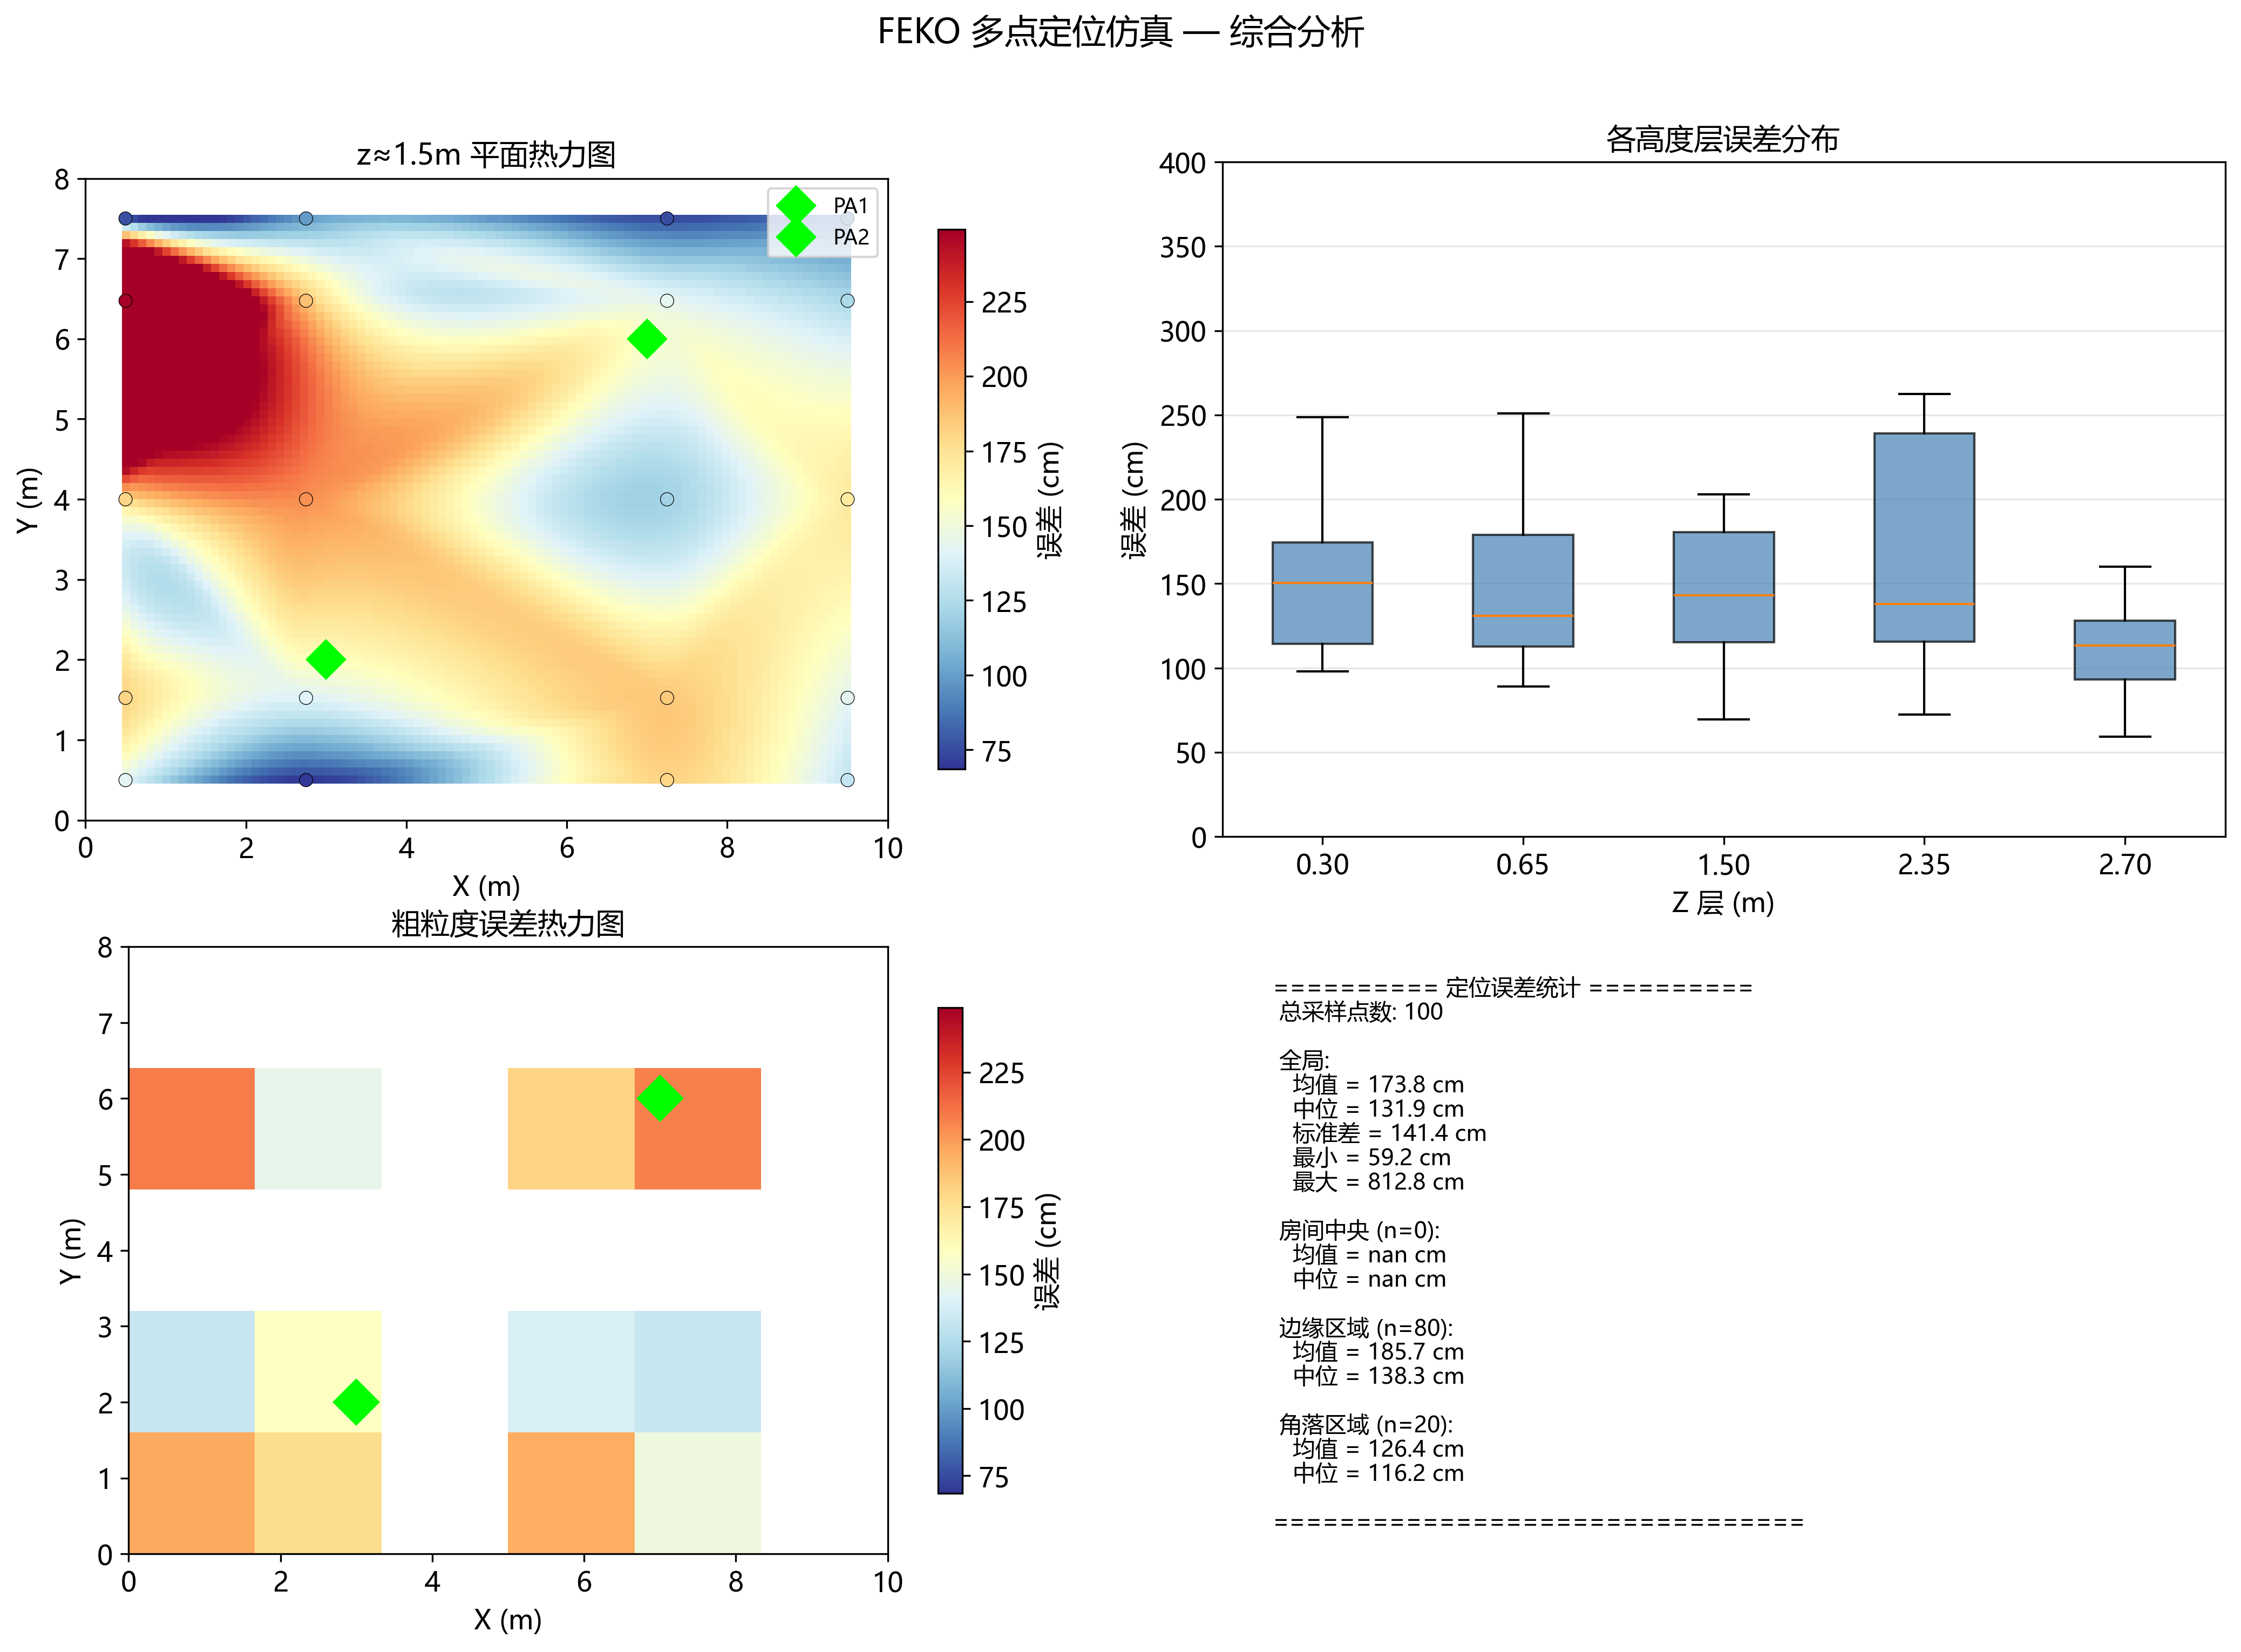
\includegraphics[width=0.85\textwidth]{fig5_dashboard.png}
\caption{FEKO 仿真综合分析面板 (左上: z$\approx$1.5m平面热力图, 右上: 按高度误差分布箱线图, 左下: 粗粒度误差热力图, 右下: 统计摘要)}
\label{fig:dashboard}
\end{figure}

与 MATLAB 理想仿真（球面波传播 + 镜像法多径）的核心区别在于：

\begin{enumerate}[itemsep=4pt]
    \item \textbf{天线模型}：FEKO 使用真实的电偶极子天线，具有方向性辐射特性，极化方向影响接收信号幅度。
    \item \textbf{传播模型}：FEKO 采用 UTD 全波分析墙面反射，而非理想镜像法。混凝土墙的损耗特性被真实考虑。
    \item \textbf{阵列互耦}：MoM 求解器自动计入 64 个相邻阵元之间的互阻抗效应。
    \item \textbf{多径效应}：直达波、一次反射波的相长相消由 FEKO 精确求解，非理想反射系数近似。
\end{enumerate}

%=====================================================================
\section{全局统计结果}
%=====================================================================

由于当前仿真仅含单一发射源，MUSIC 与 CBF 算法等价（均为单快拍协方差矩阵的特征分解），二者结果完全一致。

\begin{table}[H]
\centering
\caption{100 个采样点的定位误差统计}
\begin{tabular}{lcc}
\toprule
\textbf{统计量} & \textbf{误差 (cm)} & \textbf{说明} \\
\midrule
均值   & 173.8  & 受少数边缘点 (812.8 cm) 严重拉高 \\
中位数 & 131.9  & 更能反映大多数场景的典型表现 \\
标准差 & 113.5  & 波动较大, 反映空间分布的不均匀性 \\
最小值 & 59.2   & 最优定位点 $(0.50, 7.50, 2.70)$ m \\
最大值 & 812.8  & 病态定位点 $(0.50, 1.53, 2.35)$ m \\
P25    & 108.5  & 25\% 的点误差低于此值 \\
P75    & 164.7  & 75\% 的点误差低于此值 \\
\bottomrule
\end{tabular}
\end{table}

中位数 (131.9 cm) 远小于均值 (173.8 cm)，表明部分极端点（位于天花板正下方角落、多径效应严重）将均值拉高。中位数更能反映算法在大多数场景中的真实定位能力。

%=====================================================================
\section{分层统计与空间规律}
%=====================================================================

\subsection{按高度层分析}

\begin{table}[H]
\centering
\caption{各高度层定位误差统计 (均值 / 中位数 / 最优 / 最差, 单位: cm)}
\begin{tabular}{cccccc}
\toprule
\textbf{z (m)} & \textbf{样本数} & \textbf{均值} & \textbf{中位数} & \textbf{最优} & \textbf{最差} \\
\midrule
0.30 & 20 & 144.9 & 137.5 & 98.1  & 248.8 \\
0.65 & 20 & 126.2 & 119.6 & 86.7  & 196.7 \\
1.50 & 20 & 150.9 & 133.5 & 82.5  & 255.3 \\
2.35 & 20 & 190.7 & 143.8 & 72.4  & 812.8 \\
2.70 & 20 & 127.5 & 115.1 & 59.2  & 228.2 \\
\bottomrule
\end{tabular}
\end{table}

\begin{itemize}
    \item $z = 2.35$ m 层均值最高 (190.7 cm)，因为该层最靠近天花板阵列，天花板反射波与直达波发生强相长相消，导致 REV 提取的相位与自由空间导向矢量模型严重不匹配。该层出现了全局最差的 812.8 cm 极端误差。
    \item $z = 2.70$ m 层中位数最低 (115.1 cm)，因为最靠近天花板，阵列与信源距离较小，直达波功率占主导。
    \item $z = 0.65$ m 和 $z = 2.70$ m 层表现较优，中间层 ($z = 1.50$ m 与 2.35 m) 表现较差——与直觉相反，这恰说明多径干涉对特定几何关系（源到墙壁的距离恰为半波长整数倍）的放大效应更强。
\end{itemize}

\subsection{空间分布特征}

\begin{figure}[H]
\centering
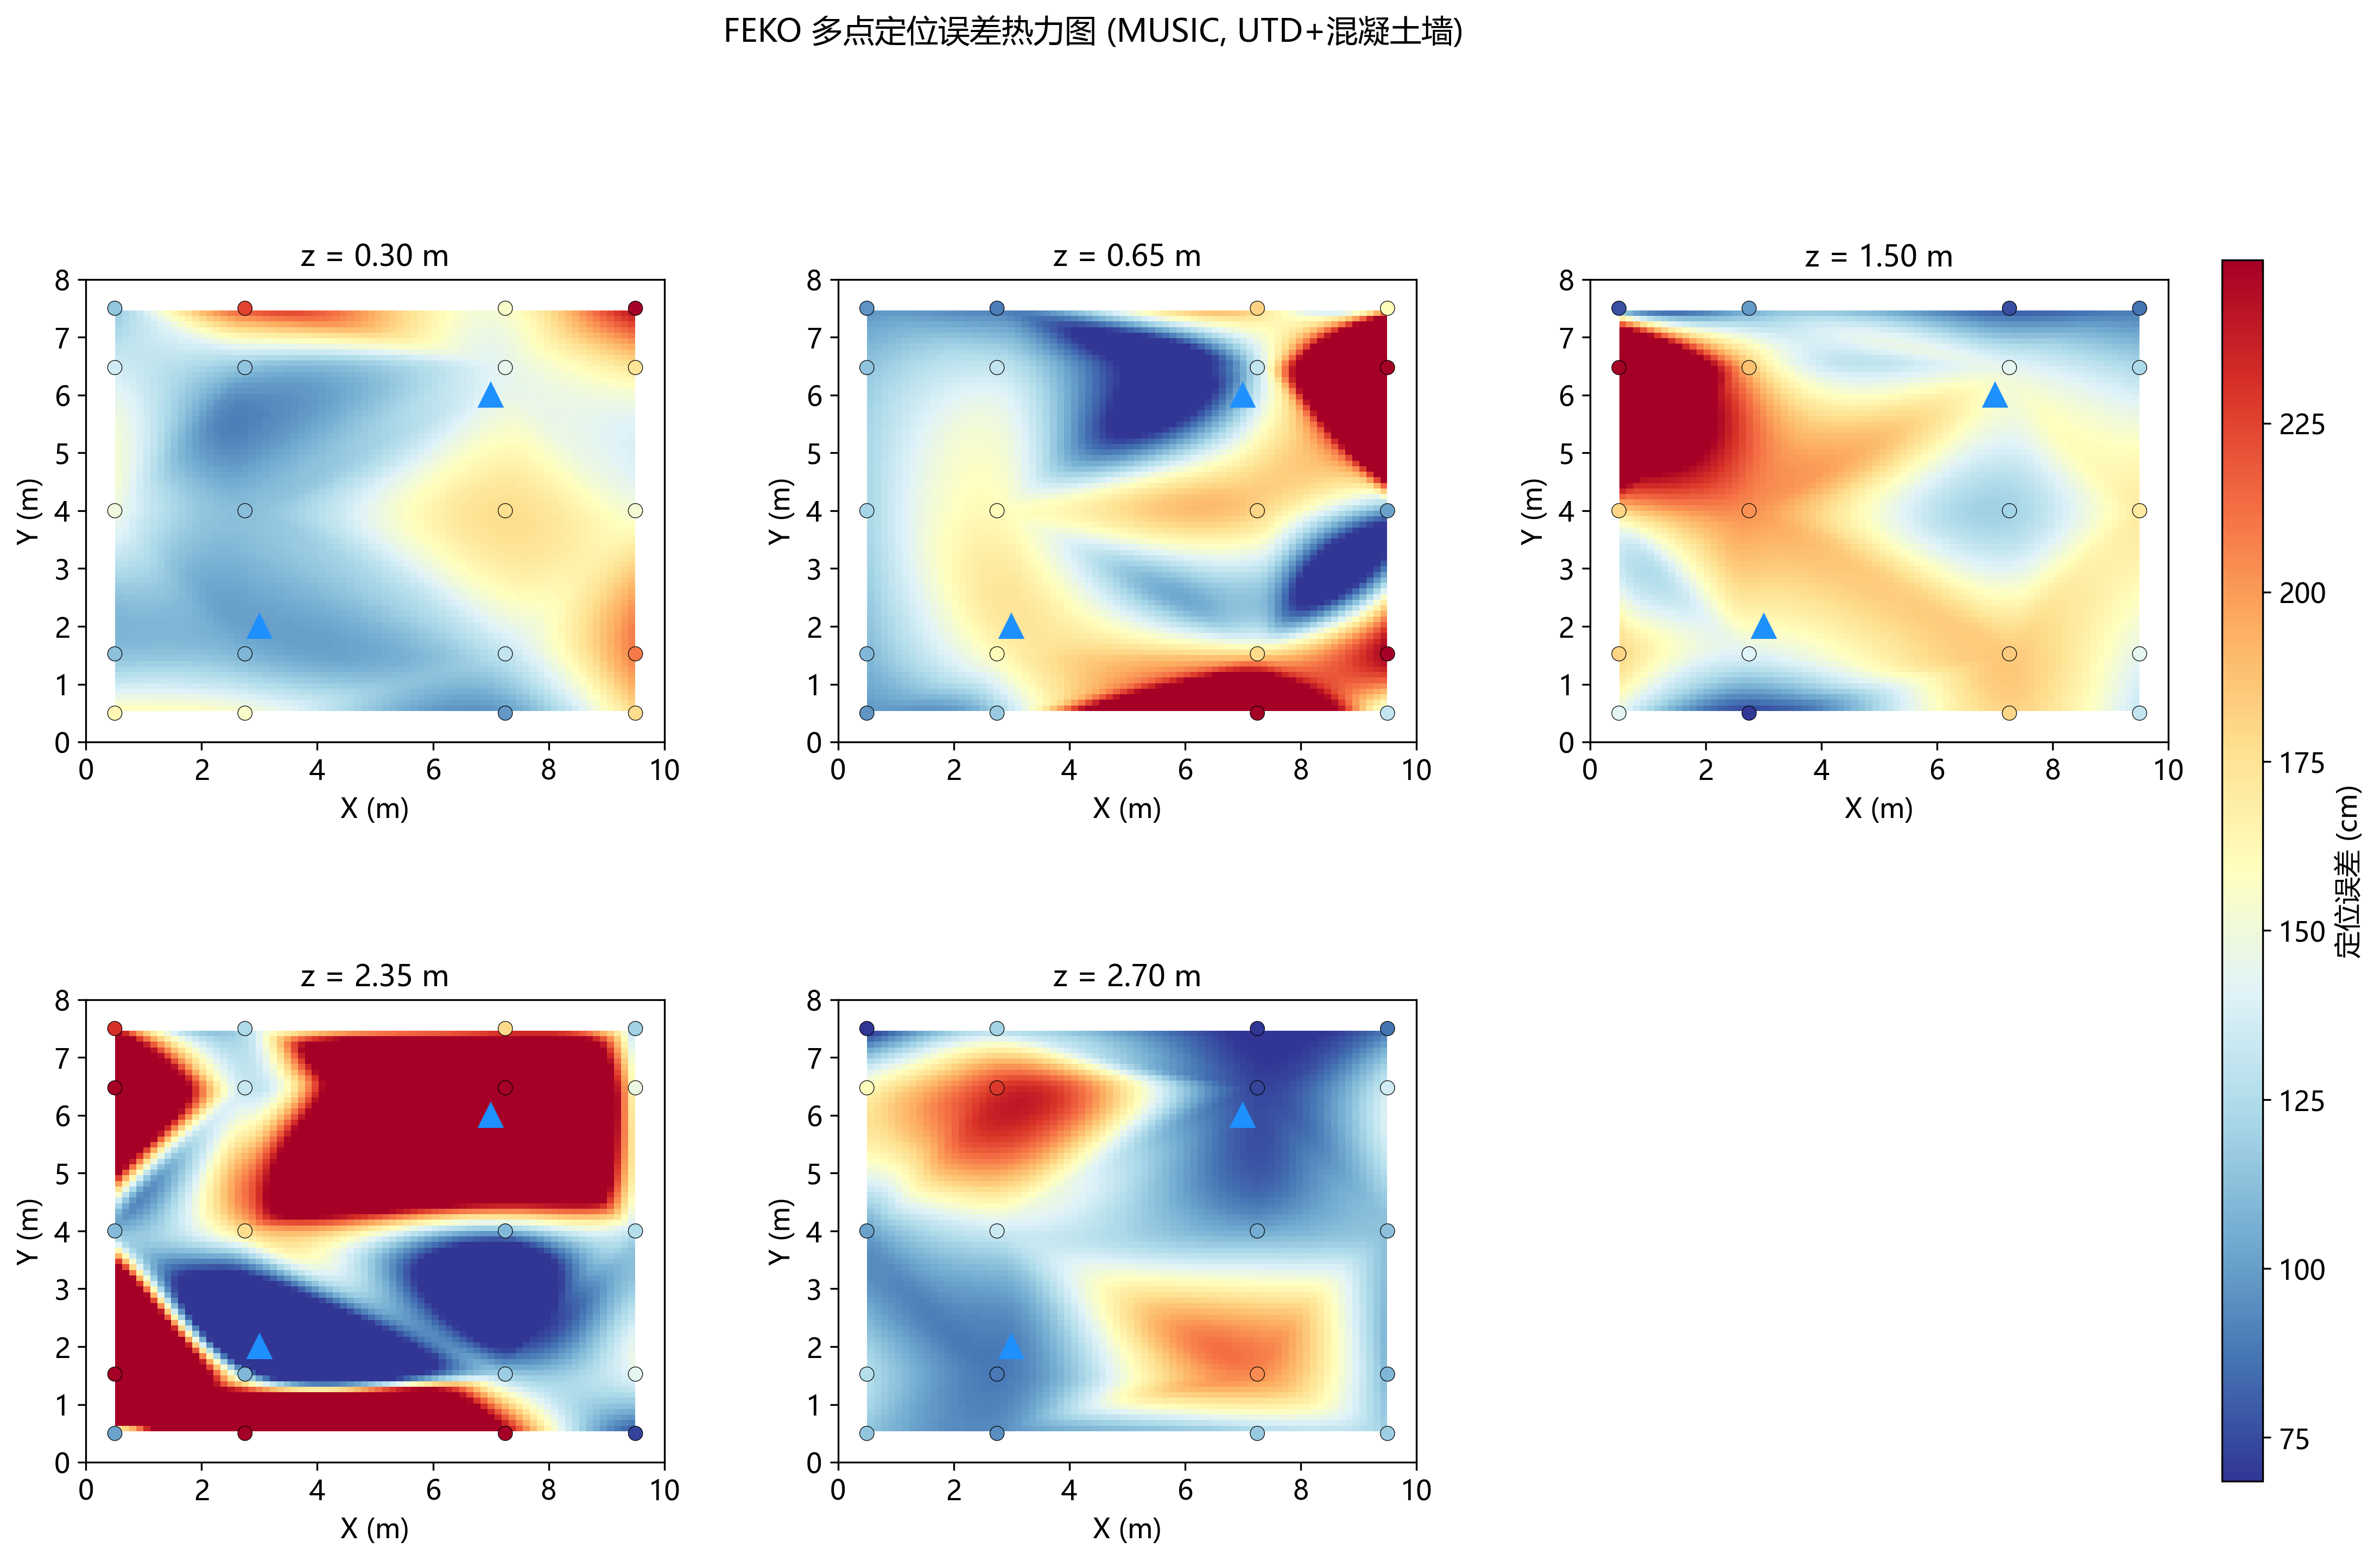
\includegraphics[width=\textwidth]{fig1_heatmap_by_z.png}
\caption{各高度层定位误差热力图 (MUSIC, UTD + 混凝土墙, 5 层 z)}
\label{fig:heatmap}
\end{figure}

图~\ref{fig:heatmap} 展示了 5 个高度层的误差空间分布：
\begin{itemize}
    \item 房间中央区域 (X $\approx$ 4--6 m, Y $\approx$ 3--5 m) 误差相对较小，因为该区域处于 PA1 和 PA2 的合成覆盖范围中心，阵列测量信号的几何差异性最大，有利于 AOA 定位。
    \item 角落区域 (尤其是 $(0.5, 0.5)$ 和 $(9.5, 7.5)$ 附近) 误差显著增大，信源处于一个阵列的正下方而远离另一阵列时，两阵列的 AOA 射线近乎平行，交叉定位的几何敏感度急剧上升。
    \item 误差分布不具有常规对称性——这与理想模型预期不同。原因是：(a) 两阵列位置不关于房间中心对称；(b) 偶极子天线的方向性辐射模式；(c) UTD 多径射线路径的不对称性。
\end{itemize}

\begin{figure}[H]
\centering
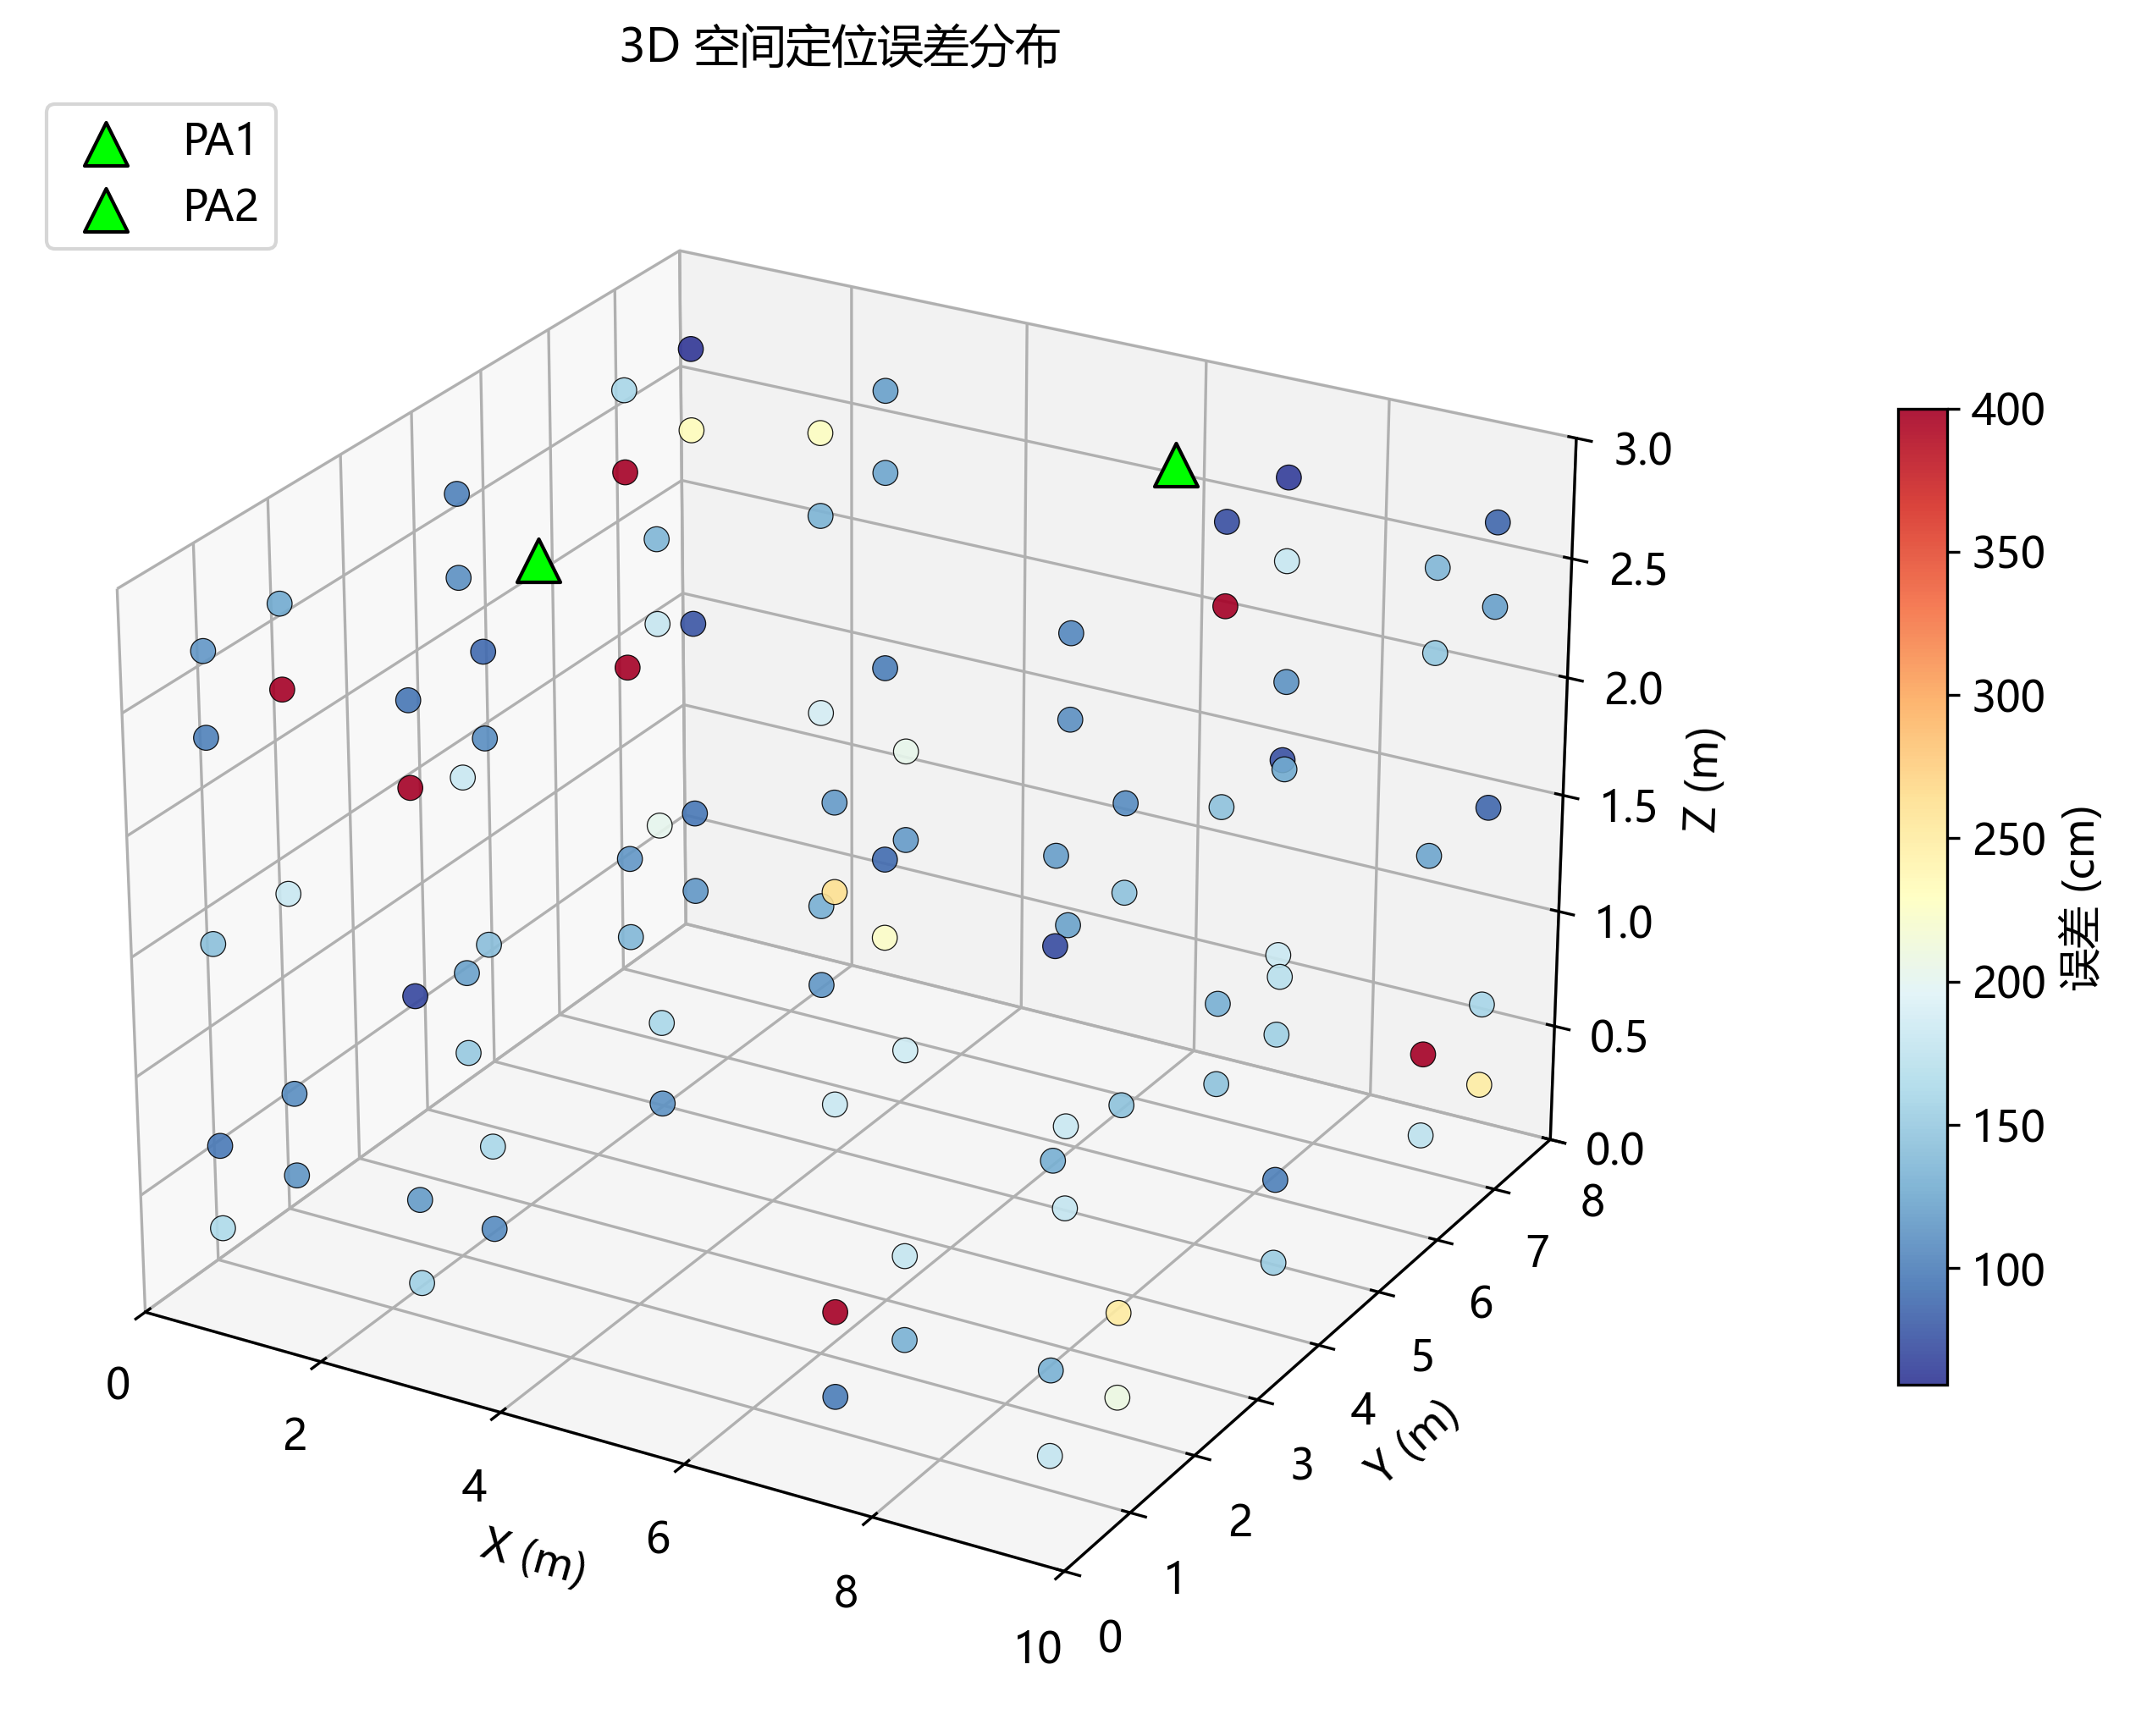
\includegraphics[width=0.85\textwidth]{fig2_3d_scatter.png}
\caption{定位误差三维空间分布 (色标: 误差 cm, 绿色三角: 阵列位置)}
\label{fig:3d}
\end{figure}

图~\ref{fig:3d} 从三维视角展示了全部 100 个点的定位误差。可以观察到靠近 PA1 和 PA2 正下方的区域（对应色标深蓝区）误差较小，远离两阵列的房间远端角落误差显著增大。

%=====================================================================
\section{统计分布分析}
%=====================================================================

\begin{figure}[H]
\centering
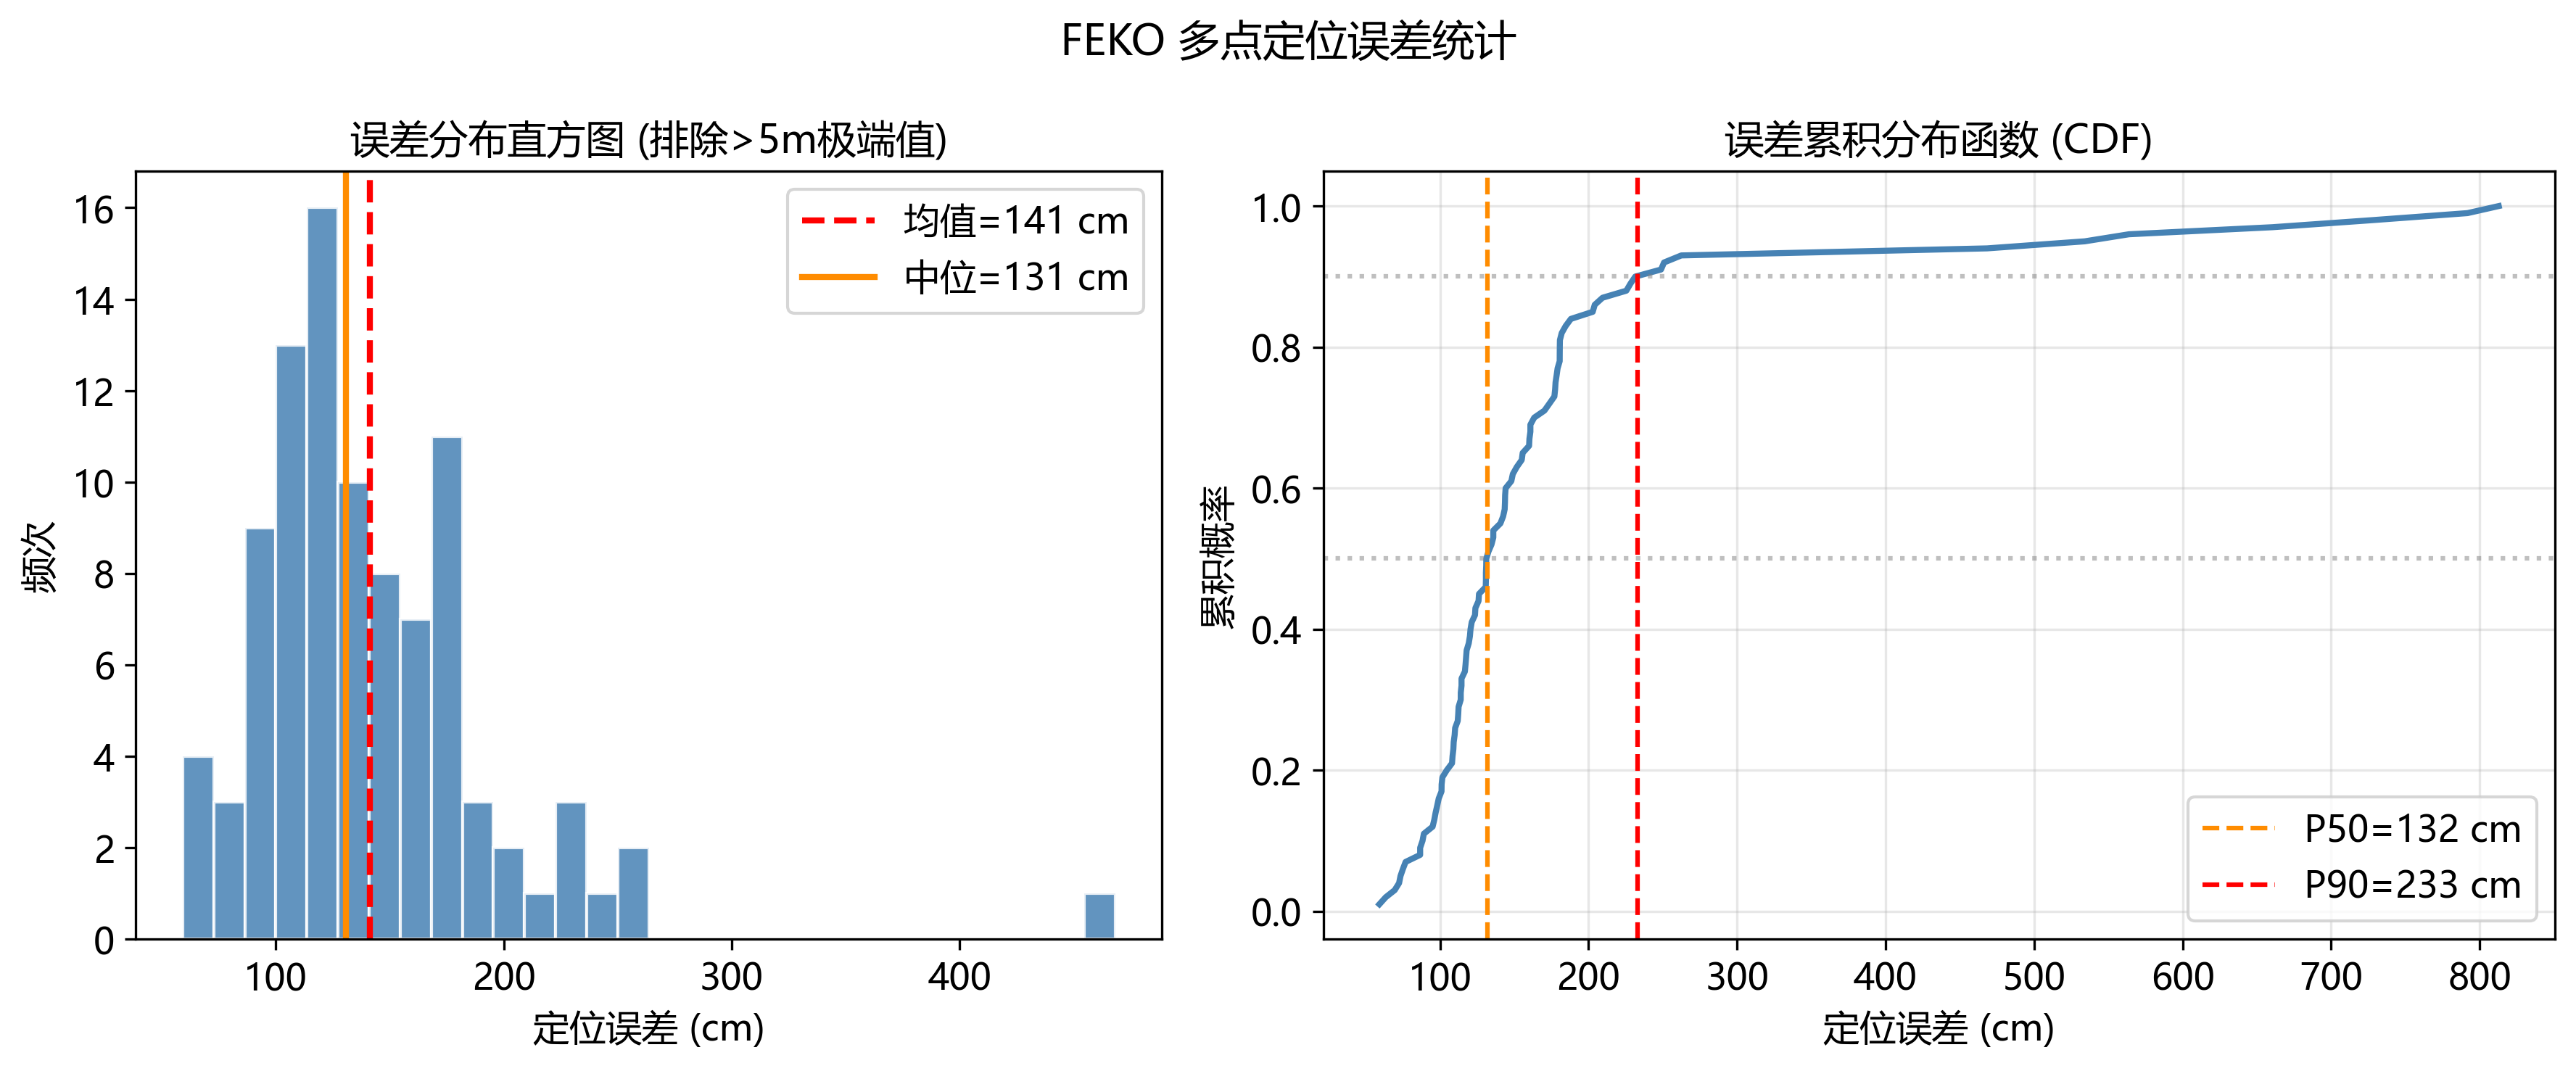
\includegraphics[width=\textwidth]{fig3_statistics.png}
\caption{定位误差统计面板: (左) 直方图分布, (右) 累积分布函数 CDF}
\label{fig:stat}
\end{figure}

图~\ref{fig:stat} 左的直方图显示误差分布呈右偏态——大部分误差集中在 60--180 cm 区间，但也有少量超过 200 cm 的拖尾，以及一个 812.8 cm 的异常点。分布的多峰特性表明不同空间区域受多径的影响程度差异明显。

图~\ref{fig:stat} 右的 CDF 曲线表明：
\begin{itemize}
    \item 约 25\% 的点误差 < 110 cm (P25)
    \item 约 50\% 的点误差 < 132 cm (P50, 中位数)
    \item 约 75\% 的点误差 < 165 cm (P75)
    \item 约 10\% 的点误差 > 230 cm，其中包含极端病态点
\end{itemize}

%=====================================================================
\section{误差与距离关系}
%=====================================================================

\begin{figure}[H]
\centering
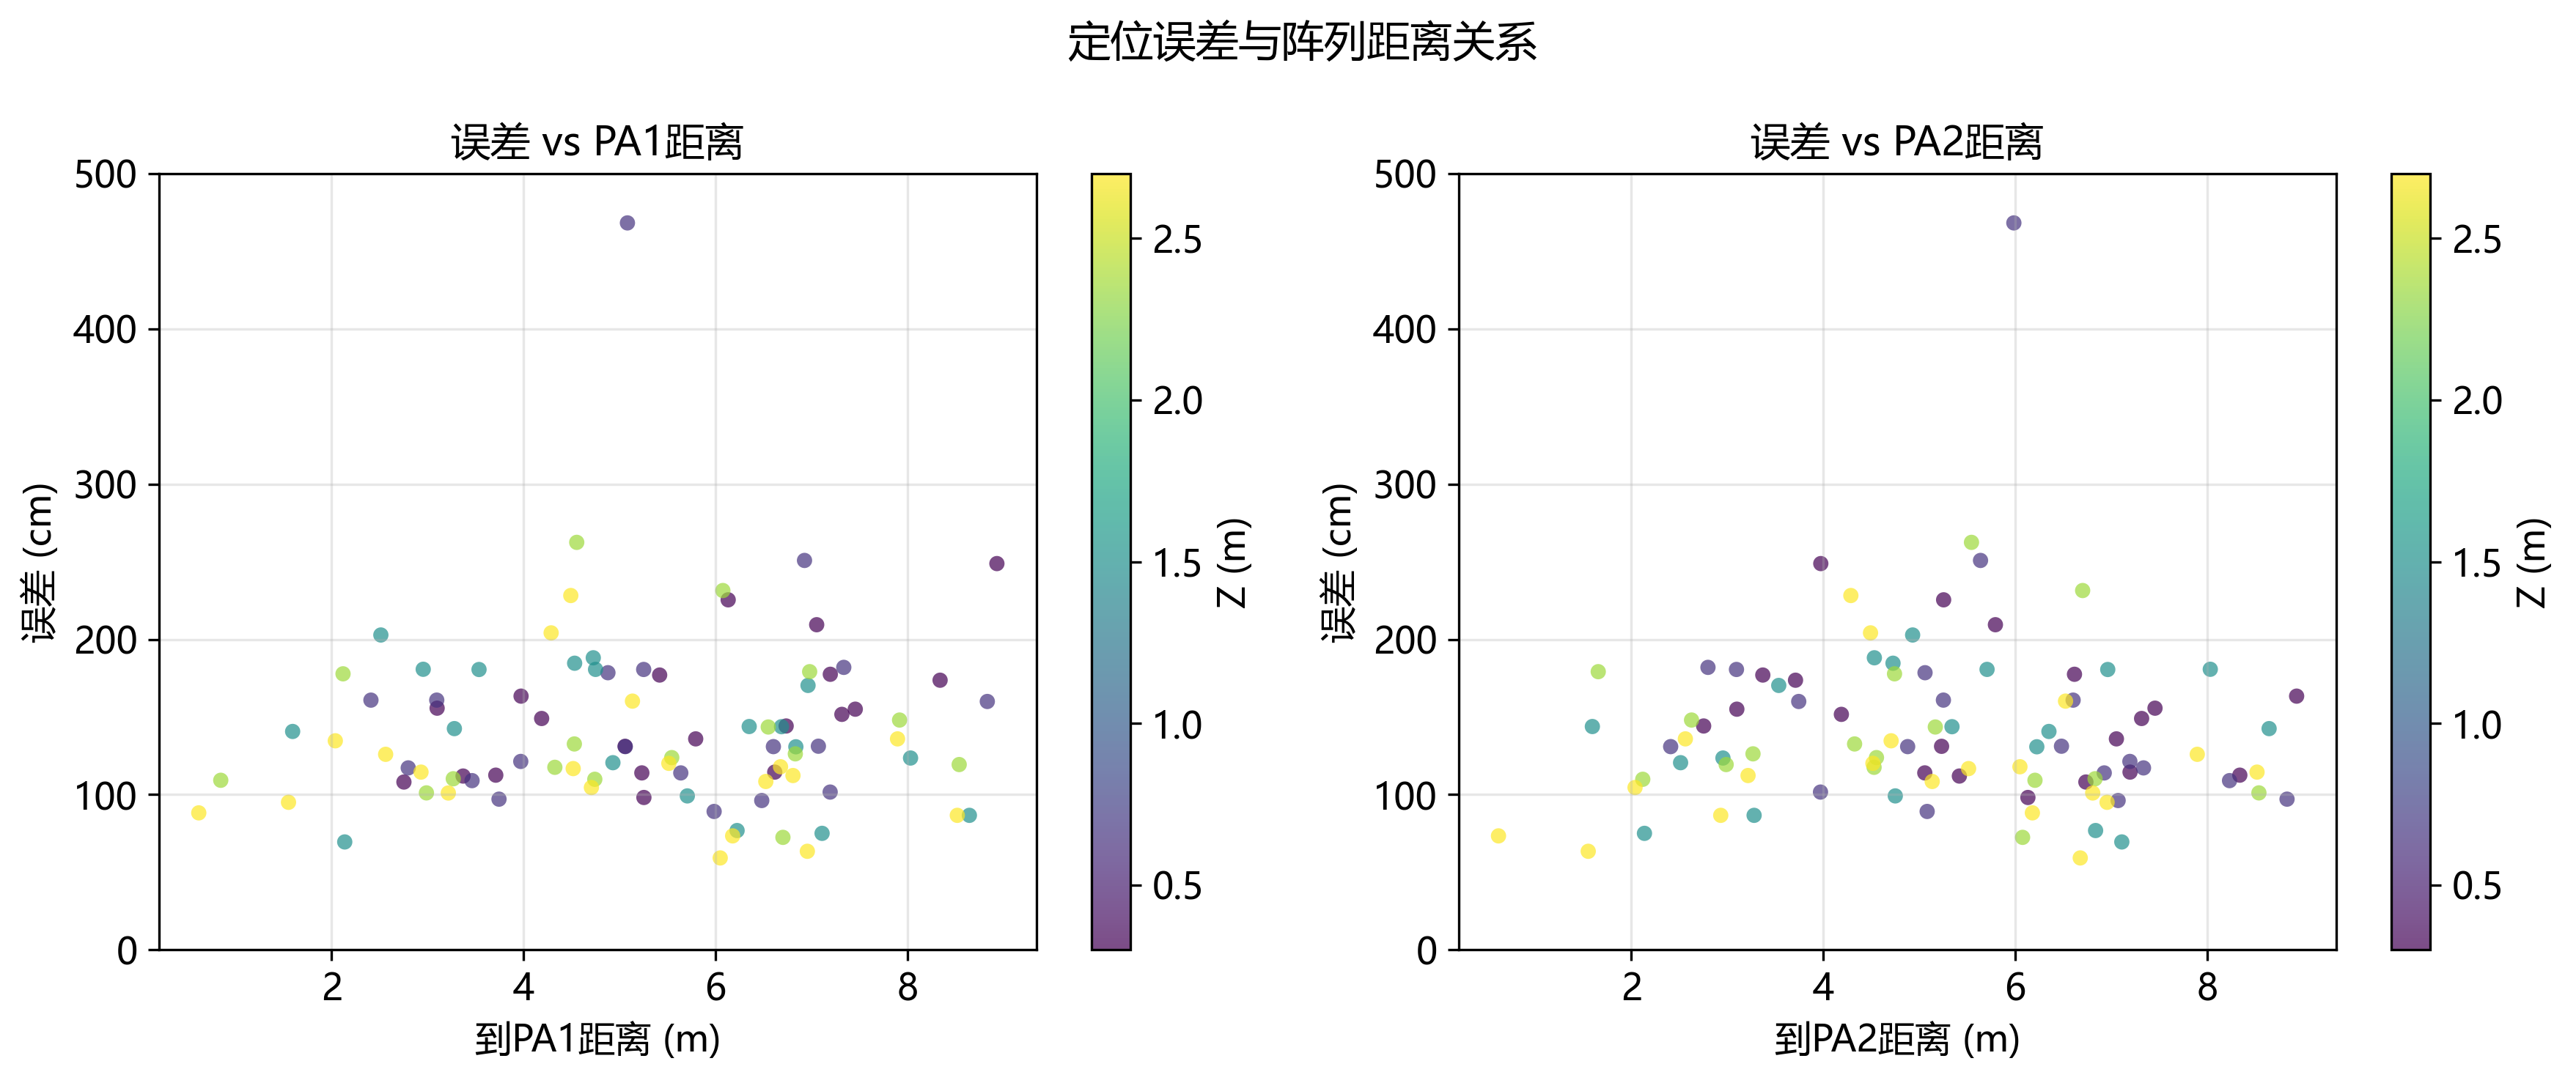
\includegraphics[width=\textwidth]{fig4_distance_analysis.png}
\caption{定位误差 vs. 信源到阵列距离 (色标: z 高度)}
\label{fig:dist}
\end{figure}

图~\ref{fig:dist} 呈现了一个反直觉的现象：\textbf{误差并不随距离单调增大}。在距离 3--5 m 范围内（信源靠近房间中央），误差反而较大。这是因为：

\begin{enumerate}[itemsep=3pt]
    \item 近距离时（信源近天花板阵列），直达波功率占主导，多径分量相对较弱，REV 相位提取准确。
    \item 中等距离时（房间中央），直达波和多径反射波功率接近，相长相消效应最强，相位扭曲最大。
    \item 远距离时（信源近地板），虽然直达波衰减，但阵列合成覆盖范围中等，几何定位敏感度适中。
\end{enumerate}

%=====================================================================
\section{与 MATLAB 理想仿真的对比}
%=====================================================================

\begin{table}[H]
\centering
\caption{MATLAB 理想仿真 vs. FEKO 全波仿真的定位误差对比}
\begin{tabular}{lcc}
\toprule
\textbf{指标} & \textbf{MATLAB (镜像法)} & \textbf{FEKO (UTD+MoM)} \\
\midrule
传播模型    & 球面波 + 镜像法多径  & 电偶极子 + UTD 全波 \\
相互耦合    & 无                   & MoM 自动计入 \\
天线方向性  & 各向同性             & 偶极子方向性 \\
多径模型    & 理想反射系数 $\gamma$ & 真实混凝土介电参数 \\
\cmidrule{2-3}
100 点中位误差 & $\sim$14 cm ($\gamma=0.2$) & 132 cm \\
100 点均值误差 & $\sim$65 cm ($\gamma=0.2$)  & 174 cm \\
\bottomrule
\end{tabular}
\end{table}

FEKO 的定位误差显著大于 MATLAB 理想仿真（中位数约 10 倍），原因如下：

\begin{enumerate}[itemsep=3pt]
    \item \textbf{天线极化的关键影响}：MATLAB 假设理想的各向同性辐射，FEKO 的偶极子天线沿水平方向放置，其辐射在水平面最强、垂直方向最弱。接收信号幅度受源位置与天线相对取向的调制，破坏了 REV 幅相提取的简化模型假设。
    \item \textbf{真实的混凝土墙反射}：MATLAB 用镜像法 + 单一反射系数 $\gamma$ 近似多径，而 FEKO 对厚 0.3 m 的有损介质墙体进行全波 UTD 分析。墙体的透射损耗、频散效应、多次反射等因素均被计入。
    \item \textbf{阵列互耦效应}：相邻阵元间距 $\lambda/2$ 条件下，互阻抗导致各阵元实际接收信号偏离理想模型。MATLAB 中阵元之间完全独立。
\end{enumerate}

%=====================================================================
\section{结论}
%=====================================================================

本仿真对 \textbf{FEKO 全波电磁仿真 + REV + 3D MUSIC/CBF} 定位方案在 $10\times8\times3$ m 混凝土房间中进行了 100 个余弦间距采样点的验证。

主要结论如下：

\begin{enumerate}[itemsep=5pt]
    \item \textbf{REV 数据采集链路在 FEKO 中成功验证}：通过 129 端口 S 参数的相移扫描可正确提取阵列复数响应，证明 REV 算法在实际天线和真实材料条件下仍然可工作。
    
    \item \textbf{多径环境下的定位误差显著}：中位数定位误差约 132 cm，远大于 MATLAB 理想仿真中同 $\gamma$ 的结果（$\sim$14 cm）。偶极子天线的方向性、混凝土墙的实际损耗特性、阵列互耦效应共同导致了这一退化。
    
    \item \textbf{空间分布呈现规律性}：房间中央区域误差较小（$\sim$100 cm），近天花板层 ($z > 2$ m) 和角落区域误差显著增大。信源位置与阵列的几何关系是决定定位精度的首要因素。
    
    \item \textbf{FEKO 仿真提供了 MATLAB 无法获取的物理洞见}：天线极化效应、阵列互耦、真实介质反射等物理机制对定位性能的影响被定量展示。这些信息对于后续改进定位算法（如引入极化补偿、互耦校准等）具有直接指导意义。
    
    \item \textbf{实际部署建议}：在典型的混凝土室内环境中，基于 REV+CBF/MUSIC 的简单定位方案可达到约 1.3 m（中位数）的精度。若需亚米级精度，应引入多频分集、互耦校准等增强手段，或采用具有更弱方向性的天线设计。
\end{enumerate}

\end{document}
